\documentclass[english]{article}
\usepackage[italian]{babel} 
\usepackage[T1]{fontenc}
\usepackage[utf8x]{inputenc}
\usepackage{float}
\usepackage{graphicx}
\usepackage{placeins}
\usepackage{wrapfig}
\includeonly{                 
./Cap1/1,
./Cap2/2,
./Cap3/3,
./Cap4/4,
./Cap5/5,
./Cap6/6,
./Appendici/A,
./Appendici/B,
./Appendici/C,
./Appendici/D
}


\makeatletter
\usepackage[a4paper,top=2cm,bottom=2cm,left=2cm,right=2cm]{geometry}
\usepackage{enumitem}
\usepackage{subfig}
\usepackage{sidecap}
\usepackage{newclude}
\usepackage{amsmath}
\usepackage{amssymb}
\usepackage{epstopdf}
\usepackage{fancyhdr}
\usepackage{booktabs,array}
\usepackage[output-decimal-marker={,}]{siunitx}
\usepackage{color}
\usepackage{empheq}
\usepackage{graphicx}
\usepackage{hyperref}
\usepackage{hf-tikz}
\usepackage{tikz}
\usetikzlibrary{spy}
\usepackage{bodegraph}
\usepackage{schemabloc}
\usetikzlibrary{circuits}
\usepackage{tabularx}
\usepackage{siunitx}
\usepackage{pgfplots, pgfplotstable}
\usepackage[siunitx]{circuitikz}
\usetikzlibrary{decorations.pathreplacing}
\usepackage[mode=buildnew]{standalone}


%%%%%%%%%%%%%% MATLAB code %%%%%%%%%%%%%%%%%%%%%%%%%%%%%%
\usepackage{listings} % inserisce listati di programmi
\definecolor{commenti}{rgb}{0.13,0.55,0.13}
\definecolor{stringhe}{rgb}{0.63,0.125,0.94}
\lstloadlanguages{Matlab}
\lstset{% general command to set parameter(s)
framexleftmargin=0mm,
frame=single,
keywordstyle = \color{blue},% blue keywords
identifierstyle =, % nothing happens
commentstyle = \color{commenti}, % comments
stringstyle = \ttfamily \color{stringhe}, % typewriter type for strings
showstringspaces = false, % no special string spaces
emph = {for, if, then, else, end},
emphstyle = \color{blue},
firstnumber = 1, % numero della prima linea
numbers =left, %  show number_line
numberstyle = \tiny, % style of number_line
stepnumber = 1, % one number_line after stepnumber
numbersep = 5pt,
language = {Matlab}, % per riconoscere la sintassi matlab
extendedchars = true, % per abilitare caratteri particolari
breaklines = true, % per mandare a capo le righe troppo lunghe
breakautoindent = true, % indenta le righe spezzate
breakindent = 30pt, % indenta le righe di 30pt
}

\DeclareMathOperator*{\rank}{rank}


% SCHEMA A BLOCCHI %
\newcommand{\trippleSpacing}{\phantom{aaa}}	% spazio di tre caratteri
\newcommand{\singleSpacing}{\phantom{a}}	% spazio di un carattere
		
\tikzstyle{block} = [draw, rectangle, minimum height=3em, minimum width=2em]
\tikzstyle{sum} = [circle, minimum width=12pt, draw, inner sep=0pt, path picture={\draw (path picture bounding box.south east) -- (path picture bounding box.north west) (path picture bounding box.south west) -- (path picture bounding box.north east);}]
\tikzstyle{input} = [coordinate]
\tikzstyle{output} = [coordinate]
\tikzstyle{pinstyle} = [pin edge={to-,thin,black}]

\tikzstyle{my right of} = [right of=#1.east]



\hyphenation{italian}
\lhead{Laboratorio di Controlli}
\rhead{Esperienza 1}

\makeatother

\usepackage{babel}








\begin{document}



\begin{titlepage} 

\begin{center}
\begin{Large} \textbf{UNIVERSITA' DEGLI STUDI DI PADOVA} \\
 \end{Large} \vspace{1cm}
 \begin{Large} \textbf{Corso di Laurea Magistrale in Ingegneria dell'Automazione}\\
 \end{Large} \vspace{2cm}
\begin{Large} Corso di Laboratorio di Controlli \end{Large}
\par\end{center}

\begin{center}
\begin{Large}Esperienza 2: Progettazione di controllori PID e con retroazione stato per un motore elettrico\\
 \end{Large}
\par\end{center}

\begin{center}
\vspace{2cm}
\begin{figure}[!htb]
\centering 
\includegraphics[width=8cm]{./figure/unipd}\\
 
\end{figure}

\par\end{center}

\begin{center}
 \vspace{2cm}
 \begin{Large} Dal Lago Nicola - 1104228 \\
 \end{Large} \vspace{2cm}
 \begin{Large} Anno Accademico 2014-2015 \end{Large} 
\par\end{center}

\end{titlepage}




\tableofcontents

\newpage
\include*{./Cap1/1}
\include*{./Cap2/2}
\section{Modellizzazione}
\label{sec:Modelizzazione}
	
	Nel corso di questa esperienza, viene impiegato un motore elettrico a corrente continua. Il motore è controllato tramite un segnale in tensione e fornisce in output l'attuale posizione del carico, attraverso l'utilizzo di un encoder.
	
	\subsection{Modellizzazione del motore}
	\label{subsec:ModellizzazioneMotore}
	
		Un motore elettrico in corrente continua, può essere suddiviso in due parti, statore e rotore. \newline
		Lo statore ha il compito di indurre un campo magnetico $B$, attraverso l'uso di materiali ferromagnetici e correnti elettriche. \newline
		Il rotore è composto da un elevato numero di spire percorse da corrente $i$ e immerse nel campo magnetico prodotto dallo statore. \newline
		Come è noto dalla \textit{legge di Faraday}, una spira in tale situazione produce una forza elettro motrice $f.e.m.$, pari all'opposto della derivata rispetto al tempo del flusso concatenato dalla spira
	
		\begin{equation}
			f.e.m. = -\frac{d\theta(t)}{dt} = AB\sin(\alpha(t))\cdot\frac{d\alpha(t)}{dt}
			\label{eq:fem}
		\end{equation}
	
		\noindent dove $A$ è l'area della spira, e $\alpha$ è l'angolo tra il vettore campo magnetico e il versore perpendicolare alla spira con verso dato dalla regola della vite destrorsa. \newline
		Si può quindi ricavare anche il momento torcente totale $\tau_{TOT}$ di ciascuna spira come
	
		\begin{equation}
			\tau_{TOT} = ABi\sin{\alpha(t)}
			\label{eq:momentoTorcente}
		\end{equation} 
	
		\noindent Riassumendo, possiamo scrivere la \textbf{dinamica elettro-meccanica} del rotore:
		
		\begin{equation}
			\begin{cases}
				f.e.m. = -AB\omega = -k_{\phi}\omega \\
				\tau_{TOT} = ABi = k_{\phi}i
			\end{cases}
			\label{eq:dinamecaElettroMeccanica}
		\end{equation}
	
		\noindent dove, con $\omega$ si indica la velocità angolare del rotore e con $k_{\phi}$ la \textit{costante elettrica} fornita da datasheet.\newline
		Per la \textbf{dinamica meccanica}, supponendo di avere un attrito viscoso descritto come $\tau_{attr} = -b\omega$, possiamo ricavarne l'equazione utilizzando il momento di inerzia $J$:
	
		\begin{equation}
			J\frac{d\omega}{dt} = k_{\phi}i - b\omega
			\label{eq:uscita}
		\end{equation}  
	
		\noindent si noti come questa equazione può essere interpretata come l'uscita del nostro sistema motore, in quanto è una equazione differenziale in funzione della velocità angolare del motore. \newline
		Passando alla \textbf{dinamica elettrica}, possiamo pensare il motore come una serie di una resistenza $R$, un generatore di forza elettromotrice $f.e.m.$ e una induttanza $L$; ai capi di tale serie, viene applicata una tensione $v_m$, il nostro controllo. Possiamo quindi scrivere l'equazione di controllo
	
		\begin{equation}
			v_m -k_{\phi}\omega = Ri + L \frac{di}{dt}
			\label{eq:controllo}
		\end{equation}    
	
		\noindent Ora possiamo unire le equazioni di uscita e di controllo, e interpretare $i$ e $\omega$ come le variabili di stato
	
		\begin{equation}
			\begin{cases}
				v_m = Ri + L\frac{di}{dt} + k_{\phi}\omega \\
				J\frac{d\omega}{dt} = -b\omega + k_{\phi}i
			\end{cases}
			\label{eq:dinamicaComplessiva}
		\end{equation}
	
		\noindent e applicando la \textit{trasformata di Laplace} scriviamo
	
		\begin{equation}
			\begin{cases}
				V_m(s) = RI(s) +sLI(s) + k_{\phi}\Omega(s)\\
				Js\Omega(s) = -b\Omega(s) + k_{phi}I(s)	
			\end{cases}
			\label{eq:dinamecaComplessivaLaplace}
		\end{equation}
	
		\noindent Con dei semplici passaggi algebrici è possibile ottenere
	
		\begin{equation}
			\Omega(s) = P(s)V_m(s) = \frac{k_{\phi}}{(R+sL)(b+SJ)+k_{\phi}}\cdot V_m(s)
			\label{eq:funzioneTrasferimento}
		\end{equation}
	
		\noindent dove con $P(s)$ indichiamo la funzione di trasferimento del processo. Nel caso del nostro motore, possiamo trascurare l'effetto induttivo, in quanto è di molto inferiore rispetto a tutti gli altri paramenti; ci risulta quindi una equazione di trasferimento
	
		\begin{equation}
			P(s) = \frac{k_{\phi}}{RJs + Rb +K_{\phi}^2}
			\label{eq:funzioneTrasferimentoSemplificata}
		\end{equation}
	
		\noindent Come accennato all'inizio del paragrafo, il motore è disposto di un encoder in grado di misurare solo la posizione angolare $\theta_m$ del motore, e non la velocità angolare; è possibile però ricondursi ad una funzione di trasferimento che abbia la posizione e non la velocità come parametro di uscita ricordando la relazione che le lega: 
	
		\begin{equation*}
			\frac{d\theta_m}{dt} = \omega
			\label{eq:posizioneVelocità}
		\end{equation*}
	
		\noindent e utilizzando la \textit{trasformata di Laplace} $s\Theta_m(s)=\Omega(s)$. Viene quindi aggiunto un polo in zero al processo:
	
		\begin{equation}
			P_{\theta}(s) = \frac{k_{\phi}}{s(RJs + Rb + k_{\phi}^2)}
			\label{eq:funzioneTrasferimentoMotoriduttore}
		\end{equation}
	
		\noindent Per comandare il motore in gradi rispetto alla tensione, bisogna introdurre due costanti moltiplicative che sono in grado di trasformare un valore in gradi a uno in tensione e viceversa:
	
		\begin{itemize}
			\item $K_{g2v}$ : costante moltiplicativa per passare da gradi a tensione;
			\item $K_{v2g}$ : costante moltiplicativa per passare da tensione a gradi.
			\label{item:costantiK} 
		\end{itemize}
	

	\subsection{Modellizzazione del motoriduttore}
	\label{subsec:ModellizzazioneMotoriduttore}
	
		Tipicamente un motore non viene usato direttamente per comandare un carico, ma si utilizzano una coppia di ingranaggi necessari per adattare le prestazioni del motore alle specifiche di progetto; questo tipo di configurazione viene chiamata \textit{motoriduzione}. E' necessario quindi definire nuove variabili:
	
		\begin{itemize}
			\item $N_m$ : numero denti dell'ingranaggio collegato al motore;
			\item $N_l$ : numero denti dell'ingranaggio collegato al carico;
			\item $\tau_m$ : momento torcente applicato al motore dall'ingranaggio;
			\item $\tau_l$ : momento torcente applicato al carico;
			\item $b_m$ : costante di attrito viscoso nel rotore lato motore;
			\item $b_l$ : costante di attrito viscoso nel rotore lato carico;
			\item $N = \frac{N_l}{N_m}$ : rapporto di motoriduzione.
		\end{itemize}  
	
		\noindent Inoltre il motore ha una serie di non idealità le quali ne complicherebbero di molto lo studio; riportiamo qui le semplificazioni fatte
	
		\begin{itemize}
			\item $L = 0$ : induttanza trascurabile;
			\item non c'è slittamento tra le ruote, il che implica;
			\begin{equation}
				\theta_mN_m = \theta_lN_l \Longrightarrow N_m\frac{d\theta_m}{dt}=N_l\frac{t\theta_l}{dt}
				\label{eq:nonIdealità1}
			\end{equation}
			\item non c'è dissipazione al punto di contatto, cioè le potenze rimangono costanti.
			\begin{equation}
				\tau_m\omega_m=\tau_l\omega_l \Longrightarrow \tau_m\frac{d\theta_m}{dt}=\tau_l\frac{d\theta_l}{dt}
				\label{eq:nonIdealità2}  
			\end{equation}
		\end{itemize}
	
		\noindent dall'equazione \ref{eq:nonIdealità1} e \ref{eq:nonIdealità2} otteniamo
	
		\begin{gather}
			\frac{\omega_m}{\omega_l}=\frac{N_l}{N_m}=N \Longleftrightarrow \omega_m=N\omega_l \\
			\tau_mN\omega_l=\tau_l\omega_l \Longleftrightarrow \tau_l=N\tau_m
		\label{gat:comp}
		\end{gather}
	
	
		\noindent e unendo tutto insieme nell'equazione del motore ricaviamo
	
		\begin{gather}
			\bigl(J_mN^2+J_l\bigl)\frac{d\omega_l}{dt}=-\bigl(b_mN^2+b_l\bigl)\omega_l+Nk_{\phi}i \\
			J_{eq}\frac{d\omega_l}{dt}=-b_{eq}\omega_l+k_{\phi,eq}i
			\label{gat:motoriduttore}
		\end{gather}
	
		\noindent Si può vedere come la forma delle equazioni del motore e del motoriduttore siano praticamente uguali, ciò che cambia è il valore delle costanti. 
		\noindent I dati di targa del motore presente in laboratorio sono riassunti nella tabella \ref{tab:parametri}. 
		
		\begin{table}[H]
			\centering
			\begin{tabular}{ccc}
				\toprule
				\textbf{Parametro} & \textbf{Valore} & \textbf{Unità di misura}\\
				\midrule
				$K_{g2v}$ & \SI{0,0284}  & $Volt/rad$       \\
				$K_{r2v}$ & \SI{1,63}    & $Volt/rad$       \\
				$N$       & \SI{14}      &                  \\
				$k_\phi$  & \SI{0,00767} & $Volt/(rad/sec)$ \\
				$J_m$     & \SI{3,87e-7} & $kg\cdot m^2$    \\ 	
				$J_l$     & \SI{3,42e-5} & $kg\cdot m^2$    \\
				$R$       & \SI{2,6}     & $\Omega$         \\
				$L$       & \SI{0,18e-3} & $H$              \\
				\bottomrule
			\end{tabular}
			\caption{Dati di targa del motore}
			\label{tab:parametri}
		\end{table}
	
		\noindent $b_m$ e $b_l$ non sono noti a priori, ma per il nostro laboratorio vengono considerati nulli, come $L$. \newline
		Come prima, anche in questo caso l'encoder ci fornisce la posizione angolare del carico e non la sua velocità, ma applicando gli stessi ragionamenti si può arrivare a formulare l'equazione finale del processo:	
		
		\begin{equation}
			P_{\theta}(s) = 
			%\tikzmarkin{right delim frac}(0.6,2.8)(-0.1,0.6)
			\frac{Nk_{\phi}}{s\bigl( R(J_mN^2+J_l) \bigl) + N^2k_{\phi}^2}
			%\tikzmarkend{right delim frac}
			\label{eq:FunzioneTrasferimentoComplessiva}
		\end{equation}
		
		\noindent mentre la vera funzione di trasferimento ``osservata'' dal motore è moltiplicata per il fattore $K_{r2v}$, risulta allora
		
		\begin{equation*}
			P_{\theta}'(s)= K_{r2v}\cdot P_{\theta}(s) \approx \frac{375}{s(s+40)}
		\end{equation*}
		
		\begin{figure}[H]
			\centering
			\subfloat[][\emph{Diagramma di Bode del modulo.}]{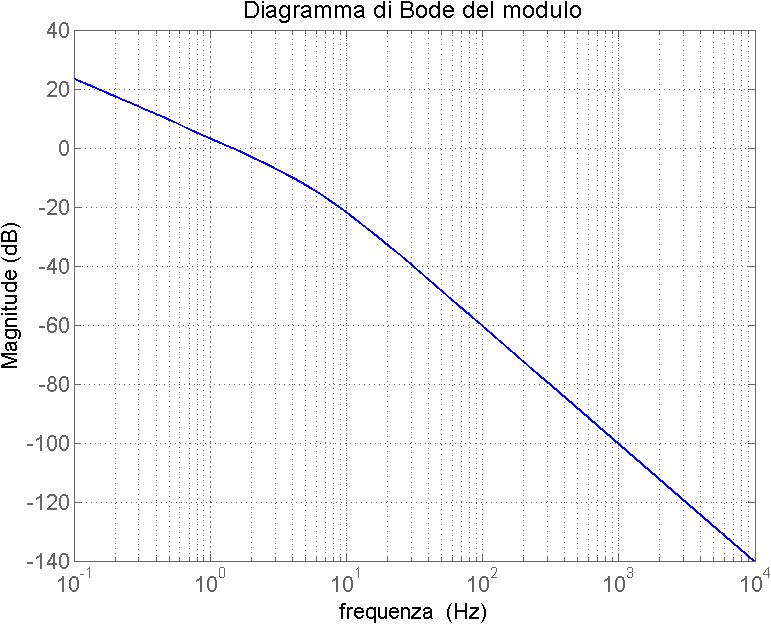
\includegraphics[width=.48\textwidth]{./figure/bode_mag.png}}\label{subfig:diagrammaBode} \quad
			\subfloat[][\emph{Diagramma di Bode della fase.}]{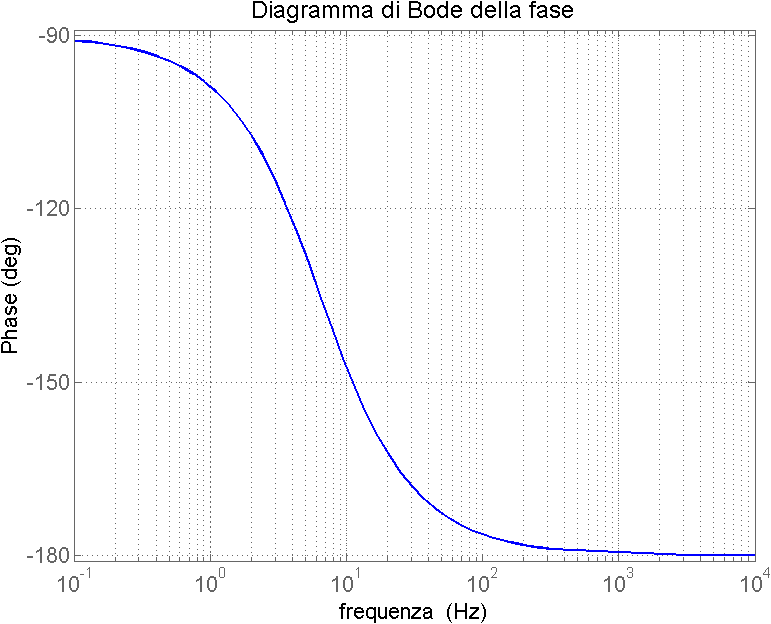
\includegraphics[width=.48\textwidth]{./figure/bode_phase.png}}\label{subfig:mappaZeriPoli}
			\caption{Diagramma di Bode di modulo e fase del processo relativo al motore.}
			\label{fig:diagrammiMotore}
		\end{figure}	
		
		\noindent In figura \ref{fig:diagrammiMotore} è rappresentato l'andamento di modulo e fase della funzione di trasferimento $P_{\theta}'(s)$.
		
	\subsection{Modellizzazione in spazio di stato}
	\label{subsec:ModelloStato}
	
	Una delle possibili rappresentazioni di un processo, insieme a quella in funzione di trasferimento usata fin'ora, è quella in spazio di stato. E' possibile scrivere il sistema come una coppia di equazioni lineari descritte come
		
	\begin{equation}
		\begin{cases}
			\dot{x}(t)=Ax(t)+Bu(t) \\
			y(t)=Cx(t)+Du(t)
		\end{cases}
	\end{equation}	
		
	\noindent dove $x(t)$ è lo stato, $u(t)$ l'ingresso e $y(t)$ l'uscita. Si dimostra che il processo in funzione di trasferimento può essere scritto come $P(s)=C(sI-A)^{-1}B+D$, ma quello che tipicamente si fa, è di ricavare direttamente le il modello dalle equazioni fisiche. Si procederà anche qui in questo modo. Le equazioni fisiche del motore, ricavate nella sessione \ref{sec:Modelizzazione}, sono divise in quattro parti:
		
	\begin{itemize}
		\item elettrica: $V_m(t)=Ri(t)+k_{\phi}^{eq}\dot{\Theta}_l$
		\item elettromeccanica: $\tau_l(t)=k_{\phi}^{eq}i(t)$
		\item meccanica: $J_{eq}\ddot{\Theta}_l=-b_{eq}\dot{\Theta}_l+\tau_l(t)$
		\item sensore: $V_{out}(t)=K_T\Theta_l$
	\end{itemize}  
		
	\noindent Come stato si è preso l'angolo del carico e la sue velocità angolare, $x=[\Theta_l \singleSpacing \dot{\Theta}_l]^T$, come ingresso $u=V_m$ e come uscita $y=V_{out}$. Si può riscrivere le prime tre equazioni nel seguente modo
		
	\begin{gather}
		i(t)=\frac{V_m(t)-k_{\phi}^{eq}\dot{\Theta}_l(t)}{R} \\
		\tau_l(t)=k_{\phi}^{eq}\Bigl(\frac{1}{R}V_m(t)-\frac{k_{\phi}^{eq}}{R}\dot{\Theta}_l\Bigl) \\
		J_{eq}\ddot{\Theta}_l=-b_{eq}\dot{\Theta}_l+\frac{k_{\phi}^{eq}}{R}V_m(t)-\frac{(k_{\phi}^{eq})^2}{R}\dot{\Theta}_l=-\Bigl(b_{eq}+\frac{(k_{\phi}^{eq})^2}{R}\Bigl)\dot{\Theta}_l(t)+\frac{k_{\phi}^{eq}}{R}V_m(t)
	\end{gather}  
		
	\noindent e allora
		
	\begin{equation}
		\begin{cases}
			\ddot{\Theta}_l(t)=-\Bigl(\frac{b_{eq}}{J_{eq}}+\frac{(k_{\phi}^{eq})^2}{R}\Bigl)\dot{\Theta}_l(t)+\frac{k_{\phi}^{eq}}{R}V_m(t) \\
			V_{out}(t)=K_T\Theta_l
		\end{cases}
	\end{equation}
		
	\noindent e riscrivendo il tutto in forma di stato esplicitando le matrici $A$, $B$, $C$ e $D$, si ottiene
		
	\begin{equation}
		\begin{cases}
			\begin{bmatrix}
				\dot{\Theta}_l(t)  \\
				\ddot{\Theta}_l(t) \\
			\end{bmatrix}
			=
			\begin{bmatrix}
				0 & 1                                  \\
				0 & -\frac{b_{eq}}{J_{eq}}-\frac{(k_{\phi}^{eq})^2}{R} \\
			\end{bmatrix}
			\begin{bmatrix}
				\Theta_l(t)       \\
				\dot{\Theta}_l(t) \\
			\end{bmatrix}	
			+
			\begin{bmatrix}
				0                       \\
				\frac{k_{\phi}^{eq}}{R} \\
			\end{bmatrix}
			V_m(t) \\
			V_{out}(t)=
			\begin{bmatrix}
				k_T & 0 \\
			\end{bmatrix}
			\begin{bmatrix}
				\Theta_l(t)       \\
				\dot{\Theta}_l(t) \\
			\end{bmatrix}
			+
			\begin{bmatrix}
				0 \\
			\end{bmatrix}
			V_m(t)											
		\end{cases}
	\end{equation}
		
	\noindent Essendo questo un sistema \textit{SISO}, la matrice di raggiungibilità ha rango pieno se e solo se il suo determinante è pari a zero. In questo caso
		
	\begin{equation}
		\mathcal{R}=[A|AB]=
		\begin{bmatrix}
			0 & \frac{k_{\phi}^{eq}}{RJ_{eq}} \\
			\frac{k_{\phi}^{eq}}{RJ_{eq}} & \star \\
		\end{bmatrix}
	\end{equation}
		
	\noindent ha rango 2, il che implica che il sistema considerato è raggiungibile. Lo stesso valo per la matrice di osservabilità
		
	\begin{equation}
		\mathcal{O}=
		\left[
		\begin{array}{cc}
			C  \\ \hline
			CA \\
		\end{array}
		\right]
		=
		\begin{bmatrix}
			k_T & 0   \\
			0   & k_T \\
		\end{bmatrix}
	\end{equation} 
		
	\noindent che ha rango pieno, il  che implica un sistema osservabile. La raggiungibilità ci garantisce che per ogni condizione iniziale, posso portare il sistema in qualunque stato. Mentre l'osservabilità ci permette di ricavare lo stato conoscendo gli ingressi e le uscite.
\section{Progettazione controllore PID con desaturatore}
\label{sec:PIDdesaturatore}

	In questa sessione si procede alla progettazione del controllore PID con desaturatore. 
	
	
	
	
	
	
	
	
	
	
	
	
	\subsection{Il controllore PID}
	\label{subsec:introduzionePID}
	
		Un controllore PID utilizza tre diverse azioni: proporzionale, integrativa e derivativa. Nella sua configurazione
		più comune esse agiscono in parallelo, cioè sono alimentate dallo stesso ingresso e le tre uscite sono poi sommate
		per ottenere l'uscita complessiva del controllore, come in Figura \ref{fig:schemaPID}. Si noti che il blocco derivatore non è un semplice $s$, ma una funzione di trasferimento strettamente propria, altrimenti impossibile da realizzare. 
	
		\begin{figure}[H]
			\centering
			\begin{tikzpicture}[auto, node distance=1.6cm,>=latex']
			
				\node [input, name=input] {};
				\node [input, name=dirama, right of=input] {};
				\node [block, right of=dirama] (kI) {$K_I$};
				\node [block, above of=kI] (kP) {$K_P$};
				\node [block, below of=kI] (kD) {$K_D$};
				\node [block, right of=kI] (I) {$\frac{1}{s}$};
				\node [block, right of=kD] (D) {$\frac{s}{1+\tau_Ls}$};
				\node [sum, right of=I] (sum) {};
				\node [output, name=output, right of=sum] {};
			
				\draw [-] (input) -- node[pos=0.05] {$e(t)$} (dirama) {};
			
				\draw [->] (dirama) |- (kP) {};
				\draw [->] (dirama) -- (kI) {};
				\draw [->] (dirama) |- (kD) {};
			
				\draw [->] (kI) -- (I) {};
				\draw [->] (kD) -- (D) {};
			
				\draw [->] (kP) -| (sum) {};
				\draw [->] (I) -- (sum) {};
				\draw [->] (D) -| (sum) {};	
			
				\draw [->] (sum) -- node[pos=0.95] {$u(t)$} (output) {};
	
			\end{tikzpicture}
			\caption{Schema a blocchi di un controllore PID}
			\label{fig:schemaPID}
		\end{figure}
	
		\noindent La funzione di trasferimento del controllore può essere scritta come:
	
		\begin{equation}
			%\tikzmarkin{right delim frac}(0.1,-0.4)(-0.1,0.6)
			C(s) = K_P + \frac{K_I}{s} + \frac{K_D s}{1 + \tau _L s}
			%\tikzmarkend{right delim frac}
			\label{eq:PID}		
		\end{equation}
	
		\noindent in cui sono presenti quattro parametri:
		\begin{itemize}
			\item $K_P$: costante dell'azione proporzionale
			\item $K_I$: costante dell'azione integrale
			\item $K_D$: costante dell'azione derivativa
			\item $\tau_L$: costante temporale legata all'azione derivativa
		\end{itemize}
	
		\noindent Si noti che in generale non è necessario utilizzare tutte e tre le azioni. Ognuna di esse infatti ha specifici effetti sulle prestazioni e sulla stabilità del sistema, schematizzate a seguire.
	
		\begin{figure}[H]
			\centering
			\begin{tikzpicture}[auto, node distance=1.6cm,>=latex']
		
				\node [input, name=input] {};
				\node [sum, right of=input] (sum) {};
				\node [block, right of=sum] (C) {$C(s)$};
				\node [block, right of=C] (P) {$P(s)$};
				\node [output, name=dirama, right of=P] {};
				\node [output, name=output, right of=dirama]  {};
				\node [output, name=fittizio, below of=C] {};
			
				\draw [->] (input) -- node[pos=0.05] {$r(t)$} node[pos=0.91] {$+$} (sum) {}; 
				\draw [->] (sum) -- (C) {};
				\draw [->] (C) -- node[pos=0.5] {$u(t)$} (P) {};
				\draw [-] (P) -- (dirama) {};
				\draw [->] (dirama) -- node[pos=0.95] {$y(t)$} (output) {};
			
				\draw [-] (dirama) |- (fittizio) {};
				\draw [->] (fittizio) -| node[pos=0.95] {$-$} (sum) {};
		
			\end{tikzpicture}
			\caption{Schema a blocchi di un classico controllo in retroazione}
			\label{fig:retroazione}
		\end{figure}
	
		\noindent Analizziamo ora gli effetti che le tre azioni del controllore portano, sia gli aspetti positivi che quelli negativi. In figura \ref{fig:retroazione} è schematizzato un classico sistema di controllo in retroazione. Definendo $G(s)=C(s)P(s)$ la funzione di trasferimento in catena aperta del sistema possiamo calcolare
	
		\begin{itemize}
			\item $\omega_a$: pulsazione di attraversamento, ovvero la pulsazione tale per cui il modulo di $G(s)$ raggiunge il valore uno;
			\item $m_{\phi}^G=180°+\arg[G(j\omega_a)]$: margine di fase, che a meno di sistemi sfortunati, da una  indicazione del grado di stabilità del sistema. Ovvero maggiore è il margine di fase, più stabile è il sistema.		 
		\end{itemize}
		
		\paragraph{Azione proporzionale P} 
	   	\label{par:P}
	   		\leavevmode\newline
	   		La parte proporzionale può essere scritta come 
	   		
	   		\begin{equation*}
	   			C_P(s)=K_P
	   		\end{equation*}
	   		
	   		\noindent Ciò porta ad avere dei diagrammi di Bode piatti, di ampiezza $20\log_{10}K_P$ dB per quanto riguarda il modulo e 0 per la fase. Questo significa che può modificare la pulsazione di attraversamento ma non il margine di fase.
	   		
	   	\paragraph{Azione integrale I}
	   	\label{par:I}
	   		\leavevmode\newline
	   		La parte integrale è invece
	   		
	   		\begin{equation*}
		   		C_I(s)=\frac{K_I}{s}
	   		\end{equation*}	
	   		
	   		\noindent Il modulo è una retta con intercetta con le ordinate pari a $20\log_{10}K_I$ dB e pendenza $-20$ dB/decade, e la fase una retta di ampiezza $-90°$. E' quindi rischioso da usare perché tende a far diventare il sistema $G(s)$ instabile, però offre il vantaggio di aggiungere un polo nell'origine e quindi di portare l'errore a regime a zero.
	   		
	   	\paragraph{Azione derivativa D}
	   	\label{par:D}
	   		\leavevmode\newline
	   		L'azione derivativa è invece
	   		
	   		\begin{equation*}
	   			C_D(s)=K_Ds
	   		\end{equation*} 
	   		
	   		\noindent In questo caso il modulo è una retta sempre con intercetta $20\log_{10}K_D$ ma con pendenza $20$ dB/decade, mentre la fase è una retta di altezza $90°$. La fase tende a far migliorare la stabilità, però la derivata del segnale amplifica il rumore in ingresso. E' necessario inoltre dire che un controllore così costruito risulta impossibile da progettare in pratica, perché avrebbe il modulo che cresce all'infinito. Quello che si fa è di aggiungere un polo in alta frequenza, facendo diventare il controllore
	   		
	   		\begin{equation*}
	   			D_D(s)=\frac{K_Ds}{1+\tau_Ls}
	   		\end{equation*} 	 
	
		\noindent I pregi e difetti delle tre azioni sono schematizzati nella tabella che segue.	
	
	
		\begin{table}[H]
			\begin{tabularx}{\textwidth}{|>{\setlength\hsize{0.6\hsize}\setlength\linewidth{\hsize}}X|>{\setlength\hsize{1.3\hsize}\setlength\linewidth{\hsize}}X|>{\setlength\hsize{1.1\hsize}\setlength\linewidth{\hsize}}X|}
			\hline
			\multicolumn{3}{|c|}{Classificazione dei tre termini del controllore in base ai pro e contro.}\\
			\hline
			Termine & Pro & Contro \\
			\hline
			\vphantom{1. Proporzionale}
			\vphantom{1. Proporzionale}
			1. Proporzionale &
			\vphantom{1. Proporzionale}
				\begin{itemize}
					\item Permette di modificare $\omega_a$ di $G(s)$ 
					\item Semplice
				\end{itemize} &
				\vphantom{1. Proporzionale}
				\begin{itemize}
					\item Non può modificare $m_\phi^G$
				\end{itemize}\\
				\hline
				\vphantom{2. Integrale}
				\vphantom{2. Integrale}
				2. Integrale &
				\vphantom{2. Integrale}
				\begin{itemize}
					\item Elimina l'errore a regime
					\item Elimina disturbi costanti in ingresso
				\end{itemize} &
				\vphantom{2. Integrale}
				\begin{itemize}
					\item Rende il sistema più instabile
				\end{itemize}\\
				\hline
				\vphantom{3. Derivativo}
				\vphantom{3. Derivativo}
				3. Derivativo &
				\vphantom{3. Derivativo}
				\begin{itemize}
					\item Rende il sistema più stabile
				\end{itemize} &
				\vphantom{3. Derivativo}
				\begin{itemize}
					\item Amplifica rumori di misura
				\end{itemize}\\
				\hline
			\end{tabularx}
			\label{tab:ProContro}
		\end{table}
	
	
	
	
	
	
	
	
	
	
	
	
	
	
	
	
	
	
	\subsection{Progettazione in frequenza del controllore PID}
	\label{sub:ProgettazionePID}
	
		Possiamo riscrivere l'equazione del PID come
		
		\begin{equation}
			C(s)=K_P + \frac{K_I}{s} + K_Ds=\frac{K_Ps+K_I+K_Ds^2}{s}=\frac{K_I(1+\frac{K_P}{K_I}s+\frac{K_D}{K_I}s^2)}{S}
			\label{eq:PIDriscritto}
		\end{equation}
		
		\noindent e definendo $\tau_I=\frac{K_P}{K_I}$ il tempo dell'azione integrale ,$\tau_D=\frac{K_D}{K_P}$ il tempo dell'azione derivativa e nell'ipotesi che $\tau_I>>\tau_D$ \footnote{Questa ipotesi è del tutto lecita, perché l'azione integrale ha appunto bisogno che l'integrale del segnale raggiunga valori significativi prima di intervenire. Mentre l'azione derivativa, soprattutto in un ingresso a gradino, agisce istantaneamente.} si ottiene 
		
		\begin{equation}
			C(s)=\frac{K_I}{s}\bigl(1+\tau_Is+\tau_D\tau_Is^2\bigl) \approx \frac{K_I}{s}\bigl(1+\tau_Is\bigl)\bigl(1+\tau_Ds\bigl)
			\label{eq:PIDtau}
		\end{equation}
		
		\noindent Aggiungendo in fine il termine di non idealità $\tau_L$ della parte derivativa e nell'ulteriore ipotesi che $\tau_I>>\tau_D>>\tau_L$ \footnote{Anche questa ipotesi è lecita, visto che il polo si cerca di metterlo più in alta frequenza possibile.}
		
		\begin{equation}
			C(s) \approx \frac{K_I(1+\tau_Is)(1+\tau_Ds)}{s(1+\tau_Ls)}
			\label{eq:PIDfinale}
		\end{equation}
	
		\noindent Perché il controllore dia i benefici desiderati, bisogna che sia soddisfatta la condizione $\tau_I>>\tau_D>>\frac{1}{\omega_a^{min}}>>\tau_L$ dove $\omega_a^{min}$ rappresenta la minima pulsazione di attraversamento richiesta nelle specifiche. Ciò comporta a scegliere
		
		\begin{equation}
			%\tikzmarkin{right delim frac}(0.1,-0.4)(-0.1,0.6)
			\tau_L=\alpha\frac{1}{\omega_a^min} \singleSpacing, \trippleSpacing \frac{1}{3}\le\alpha\le\frac{1}{10}
			%\tikzmarkend{right delim frac}
			\label{eq:tauL}
		\end{equation}
		
		\noindent Si definisce poi 
		\begin{equation}
			a=\frac{1}{|P(j\omega_a)|} \trippleSpacing \trippleSpacing \trippleSpacing \theta=\arg\bigl[C(j\omega_a)\bigl]=m_{\phi}^G-180°-\arg\bigl[P(j\omega_A)\bigl]
		\end{equation}
	
		\noindent e riscrivendo la funzione di trasferimento del controllore nella variabile $j\omega$
		
		\begin{equation}
			C(j\omega_a)=K_P-j\frac{K_I}{\omega_a}+j\omega_aK_D=K_P+j\bigl(\omega_aK_D-\frac{K_I}{\omega_a}\bigl)
		\end{equation}
		
		\noindent si ottiene
		
		\begin{align}
			\Re\Bigl[C(j\omega_a)\Bigl] &= a\cos\theta=K_P \\
			\Im\Bigl[C(j\omega_a)\Bigl] &= a\sin\theta=\omega_aK_D-\frac{K_I}{\omega_a}
			\label{eq:asen}
		\end{align}
	
		\noindent L'equazione \ref{eq:asen} mi fornisce un grado di libertà nella scelta dei parametri $K_P$ e $K_D$, tenendo però conto di soddisfare $\tau_I>>\tau_D$. Solitamente si sceglie 
		
		\begin{equation}
			\tau_I=b\tau_D \singleSpacing, \trippleSpacing b\ge4
		\end{equation}
	
		\noindent stando attenti a non scegliere $b$ troppo grande, altrimenti avrei tempi di reiezione del disturbo troppo lunghi. Rimane solo da ricavare $K_I$, per fare ciò basta risolvere l'equazione
		
		\begin{equation}
			K_Ia\sin\theta=\omega_a\frac{K_P^2}{b}-\frac{K_I^2}{\omega_a}
		\end{equation}
	
		\noindent con $K_I$ incognita. Risolvendola si otterranno due valori, ma a noi interessa solo quello positivo e quindi
		
		\begin{equation}
			K_I=\frac{a\omega_a}{2}\Biggl[\sqrt{\sin^2\theta+\frac{4}{b}\cos^2\theta}-\sin\theta\Biggl]
		\end{equation}
		
		\noindent e allora
		
		\begin{equation}
			K_D=\frac{K_P^2}{bK_I}
		\end{equation}
		
		\noindent In questo caso però, le specifiche richieste non sono fornite in frequenza, ma in termini temporali. 
		
		\begin{align}
			t_s &\le 30 \singleSpacing \textrm{[s] rispetto a $\pm1$ [gradi] dal valore a regime} \\
			S   &\le 5 \singleSpacing \textrm{[gradi]}
			%r   &= 10,\singleSpacing 50, \singleSpacing 120 \singleSpacing \textrm{[gradi]} \\
			%d   &= \pm0.5 \singleSpacing \textrm{[Volt]}  
		\end{align}
		
		\noindent Il tempo di assestamento viene trasformato in un limite alla banda passante minima che il sistema deve garantire. Visto che si considera un sistema del secondo ordine, è possibile approssimare la banda passante con la frequenza di taglio $\omega_a$ e ottenere:
		
		\begin{equation}
			\omega_a^{min}= \frac{3}{\xi t_{s,max}}
		\end{equation}
		
		\noindent dove $\xi$ rappresenta il coefficiente di smorzamento. Il vincolo sul massima sovraelongazione invece può essere convertito in una richiesta sul minimo margine di fase $m_{\phi}$ ammissibile. Per la conversione si possono allora utilizzare i due grafici riportati in figura \ref{fig:mSxiS}. Per una spiegazione dettagliata su come si possono ricavare i due grafici è possibile consultare l'appendice ?????.
		
		\begin{figure}[H]
			\centering
			\begin{tikzpicture}[scale=1]
				\begin{axis}[grid=both, xlabel=\phantom{$m_{\phi}^G$} $\xi$ \phantom{$m_{\phi}^G$}, ylabel=$S\singleSpacing \%$,enlargelimits=false]
			    	\addplot[domain=0:1, blue, ultra thick] {100*e^((-3.14*x)/(1-x^2)^(1/2)};
				\end{axis}
			\end{tikzpicture}
			\begin{tikzpicture}[scale=1]
				\begin{axis}[grid=both, xlabel=$m_{\phi}^G$, ylabel=$S\singleSpacing \%$,enlargelimits=false]
			    	\addplot[domain=0:90, blue, ultra thick] {100*e^((-3.14*(tan(x)/(16*(tan(x))^2+16)^(1/4)))/((1-((tan(x)/(16*(tan(x))^2+16)^(1/4)))^2)^(1/2)))};
				\end{axis}
			\end{tikzpicture}
			\caption{Relazione tra $m_{\phi}$ e $S$ e tra $\xi$ e $S$.}
			\label{fig:mSxiS}
		\end{figure}
		
		
		
		
		
		
		
	
	
	
	
	
	
	
	
	
	
	
		
		
	\subsection{Progetto del controllore PID con desaturatore}
	\label{subsec:Desaturatore}
	
		\begin{figure}[H]
			\centering
			\begin{tikzpicture}[auto, node distance=1.6cm,>=latex']
				\node [input, name=input] {};
				\node [sum, right of=input] (sum1) {};
				\node [input, name=dirama1, right of=sum1] {};
				\node [block, right of=dirama1] (D) {$K_D\frac{s}{1+\tau_Ls}$};	
				\node [block, above of=D] (P) {$K_P$};
				\node [block, below of=D] (I) {$\frac{K_I}{s}$};
				\node [sum, below of=dirama1] (sum2) {};
				\node [sum, right of=D] (sum3) {};
				\node [input, name=dirama2, right of=sum3] (dirama2) {};
				\node [block, right of=dirama2] (saturatore) {saturatore};
				\node [input, name=dirama3, right of=saturatore] {};
				\node [block, right of=dirama3] (Ps) {$P(s)$};
				\node [input, name=dirama4, right of=Ps] {};
				\node [output, name=output, right of=dirama4] {};
				\node [sum, below of=dirama2] (sum4) {};
				\node [input, name=fittizio, below of=sum4] {};	
				\node [block, left of=fittizio] (Ka) {$K_a$};
				\node [input, name=fittizio2, below of=Ka] {};

				\draw [->] (input) --  node[pos=0.05] {$r(t)$}  node[pos=0.91] {$+$} (sum1) {};
				\draw [-] (sum1) --  node[pos=0.3] {$e(t)$} (dirama1) {};
				\draw [->] (dirama1) |- (P) {};
				\draw [->] (dirama1) -- (D) {};
				\draw [->] (dirama1) --  node[pos=0.95] {$+$} (sum2) {};
				\draw [->] (P) -| (sum3) {};
				\draw [->] (D) -- (sum3) {};
				\draw [->] (I) -| (sum3) {};
				\draw [->] (sum2) -- (I) {}; 
				\draw [-] (sum3) --  node[pos=0.5] {$u_{PID}(t)$} (dirama2) {};
				\draw [->] (dirama2) -- (saturatore) {};
				\draw [-] (saturatore) --  node[pos=0.6] {$u(t)$} (dirama3) {};
				\draw [->] (dirama3) -- (Ps) {};
				\draw [-] (Ps) -- (dirama4) {};
				\draw [->] (dirama4) --  node[pos=0.95] {$y(t)$} (output) {};
				\draw [->] (dirama2) --  node[pos=0.95] {$+$} (sum4) {}; 	
				\draw [-] (sum4) -- (fittizio) {};	
				\draw [->] (fittizio) -- (Ka) {};
				\draw [->] (Ka) -|  node[pos=0.95] {$-$} (sum2) {};
				\draw [->] (dirama3) |-  node[pos=0.95] {$-$} (sum4) {};	
				\draw [-] (dirama4) |- (fittizio2) {};
				\draw [->] (fittizio2) -|  node[pos=0.98] {$-$} (sum1) {};
			\end{tikzpicture}
			\caption{Schema a blocchi di un controllore PID con desaturatore}
			\label{fig:PIDdesaturatore}
		\end{figure}
	
		\noindent Il motore utilizzato in laboratorio è comandato con un segnale di tensione, tale segnale deve essere compreso tra un intervallo di valori pari a $[-5,5]$ Volt. Ciò significa che è necessario saturare il segnale di controllo con un dispositivo denominato saturatore. Saturando l'ingresso al motore, l'errore $e(t)$ che comanda il controllore tende a diminuire più lentamente e il suo integrale sarà allora maggiore. Questo vuol dire che amplifica l'azione integrale durante la saturazione, rendendo il sistema più instabile. Per ovviare a questo introduco un secondo controllo in retroazione che interviene solo in caso di saturazione, lo schema di tale controllo è presente in Figura \ref{fig:PIDdesaturatore}. Questa retroazione diminuisce il termine integrale per un fattore proporzionale alla differenza tra l'uscita del controllore e la vera uscita che riceve il motore. Rimane quindi da scegliere la variabile $K_a$. Con qualche passaggio algebrico è possibile scrivere la funzione di trasferimento tra l'uscita del controllore $U_{PID}(s)$ e l'errore $E(s)$ in presenza di saturazione come   
	
		\begin{equation}
			U_{PID}(s)=\frac{K_P+K_Ds+\frac{K_I}{s}}{1+\frac{K_aK_I}{s}}E(s)
			\label{eq:Upid}
		\end{equation}
	
		\noindent Si vede dall'equazione \ref{eq:Upid} che il parametro $K_a$ introduce un filtro passa basso che tende a rallentare il controllo. Allora si definisce la costante temporale del desaturatore $\tau_a=K_aK_I$ e quello che si vuole è che $\tau_a<t_r$. Tipicamente si sceglie
		
		\begin{equation}
			\tau_a \approx \frac{1}{3}t_r \trippleSpacing \Rightarrow \trippleSpacing K_a \approx \frac{1}{3t_rK_I}
		\end{equation}
\section{Progettazione controllori in spazio di stato}
\label{sec:spazioDiStato}	

	In questa sessione si procede alla realizzazione di due tipi di controllori in spazio di stato.
	
	
		
	\subsection{Controllo in feedforward}
	\label{sub:feedforward}
		
		La rappresentazione in spazio di stato permette di fare una retroazione di stato invece che una retroazione dell'uscita, ed è proprio quello che si fa nel \textit{controllo in feedforward}. 
		
		\begin{figure}[H]
			\centering
			\begin{tikzpicture}[auto, node distance=2cm,>=latex']
				\node [input, name=input] {};
				\node [block, right of=input] (N) {$\bar{N}$};
				\node [sum, right of=N] (sum) {};
				\node [block, right of=sum] (xd) {$\dot{x}=Ax+Bu$};
				\node [block, below of=xd] (u) {$u=Kx$};
				\node [input, name=dirama, right of=xd] {};
				\node [block, right of=dirama] (y) {$y=Cx+Du$};
				\node [output, name=output, right of=y] {};
				
				\draw [->] (input) -- node[pos=0.05] {$r(t)$} (N) {};
				\draw [->] (N) -- node[pos=0.4] {$u_{ext}(t)$} node[pos=0.95] {$+$} (sum) {}; 
				\draw [->] (sum) -- node[pos=0.4] {$u(t)$} (xd) {};
				\draw [-] (xd) -- node[pos=0.5] {$x(t)$} (dirama) {};
				\draw [->] (dirama) |- (u) {};
				\draw [->] (u) -| node[pos=0.95] {$-$} (sum) {};
				\draw [->] (dirama) -- (y) {};
				\draw [->] (y) -- node[pos=0.95] {$y(t)$} (output) {};	
			\end{tikzpicture}
			\caption{Schema a blocchi di un controllo in feedforward.}
			\label{fig:feedforward}
		\end{figure}
		
		\noindent Con una retroazione dallo stato, il controllo, e quindi la matrice $K$, viene scelta piazzando i poli in catena chiusa del sistema. Ricordando che un processo può essere scritto in forma di stato come $P(s)=C(sI-A)^{-1}B$, si nota immediatamente che i poli corrispondono agli autovalori  di $sI-A$. Nel sistema complessivo retroazionato, tali autovalori sono di $sI-A+BK$. Il controllo in feedforward, oltre al piazzamento dei poli permette di modificare anche un parametro scalare $\bar{N}$. Per comprendere lo scopo del parametro $\bar{N}$, si pensi di voler riuscire ad inseguire perfettamente un segnale di ingresso costante:
		
		\begin{align*}
			&r(t)=cost \implies y_{DC}=cost \\
			&y_{DC}=P_{CC}(0)r=-C(A-BK)^{-1}Br
		\end{align*} 
		
		\noindent Per sistemi \textit{SISO} $-C(A-BK)^{-1}B$ si riduce ad uno scalare $c$ per cui $y=cr$ e quindi per poter inseguire il riferimento si usa in blocco $\bar{N}$ che cancella il termine $c$. $\bar{N}$ sarà allora scelto nel seguente modo
		
		\begin{equation}
			\bar{N} = \frac{1}{-C(A-BK)^{-1}B}
			\label{eq:Nbarra}
		\end{equation}
		
		\noindent Un possibile problema di questo tipo di controllo è che se non si conoscono perfettamente i valori nominali delle matrici $(A,B,C,D)$, a regime non si riesce ad inseguire perfettamente il riferimento, perchè
		
		\begin{equation}
			y_{DC}=\bar{N}[-C(A-BK)^{-1}B]r_{DC}=\frac{C(A-BK)^{-1}B}{C_{nom}(A_{nom}-B_{nom}K)^{-1}B_{nom}}r_{DC} \ne r_{DC}
		\end{equation}
		
		\noindent Un altro problema è se è presente un disturbo additivo $d(t)$ in ingresso al controllo, infatti risulterebbe
		
		\begin{equation}
			y_{DC}=\alpha r_{DC} + \beta d_{DC}
		\end{equation} 
		
		
		
		
		
		
		
	\subsection{Controllo integrale}
	\label{subsec:ControlloIntegrale}
	
		\begin{figure}[H]
			\centering
			\begin{tikzpicture}[auto, node distance=1.45cm,>=latex']
				\node [input, name=input] {};
				\node [sum, right of=input] (sum1) {};
				\node [block, right of=sum1] (int) {$\int dt$};
				\node [block, right of=int] (kI) {$K_I$};
				\node [sum, right of=kI] (sum2) {};
				\node [output, name=fittizio3, right of=sum2]{};
				\node [sum, right of=fittizio3] (sum3) {};
				\node [output, name=fittizio0, right of=sum3]{};
				\node [block, right of=fittizio0] (sistema){$\dot x=Ax+Bu$};
				\node [input, name=disturbo, above of=sum3] {};
				\node [block, below of=sum3] (K) {$K$};
				\node [output, name=fittizio, below of=K] {};
				\node [output, name=dirama1, right of=sistema] {};
				\node [block, right of=dirama1] (C){$y=Cx$};
				\node [output, name=dirama2, right of=C] {};
				\node [output, name=output, right of=dirama2] {};
			
				\draw [->] (input) -- node[pos=0.05] {$r(t)$} node[pos=0.95] {$+$}(sum1) {};
				\draw [->] (sum1) -- node[pos=0.5] {$e(t)$} (int) {};
				\draw [->] (int) -- node[pos=0.5] {$-x_I$}(kI) {};
				\draw [->] (kI) -- node[pos=0.95] {$+$} (sum2) {};
				\draw [-] (sum2) --  node[pos=0.95] {$u_{ext}(t)$} (fittizio3) {};
				\draw [->] (fittizio3) -- node[pos=0.95] {$+$}(sum3){};
				\draw [->] (disturbo) -| node[pos=0.05] {$d(t)$} node[pos=0.95] {$+$} (sum3){};
				\draw [-] (sum3) -- node[pos=0.5] {$u(t)$}(fittizio0){};
				\draw [->] (fittizio0) -- (sistema){};
				\draw [-] (sistema) -- (dirama1){};
				\draw [->] (dirama1) -- node[pos=0.3] {$x(t)$} (C){};
				\draw [->] (dirama1) |- (K){};
				\draw [->] (K) -| node[pos=0.95] {$-$}(sum2){};
				\draw [-] (C) -- (dirama2){};	
				\draw [->] (dirama2) -- (output) {};
 				\draw [-] (dirama2) |- (fittizio){};
 				\draw [->] (fittizio) -| node[pos=0.95] {$-$} (sum1){}; 
				\draw [->] (C) -- node[pos=0.95] {$y(t)$}(output){};	
			\end{tikzpicture}
			\caption{Schema a blocchi di un controllo integrale con rumore additivo $d(t)$}
			\label{fig:integrale}
		\end{figure}	
	
		\noindent Il controllo integrale è un altro esempio di controllore che sfrutta la retroazione di stato. Prendiamo in considerazione un sistema scritto in forma di stato, dove per semplicità si considera nulla la matrice $D$ \footnote{del tutto lecito visto che il sistema del motore ha appunto $D=0$}
		
		\begin{equation}
			\begin{cases}
				\dot{x}=Ax+Bu \\
				y=Cx
			\end{cases}
			\label{eq:sistemaNoD}
		\end{equation}
	
		\noindent Al sistema viene aggiunto un nuovo stato
		
		\begin{equation}
			\dot{x}_I=e=y-r=Cx-r
			\label{eq:NuovoStato}
		\end{equation}
	
		\noindent ottenendo ancora un sistema dinamico. Si definisce allora un nuovo \textit{stato aumentato} $z \in \mathbb{R}^{n+1}$
		
		\begin{equation}
			z=
			\begin{bmatrix}
				x_I \\
				x
			\end{bmatrix}
			\label{eq:statoAumentato}
		\end{equation}
	
		\noindent e supposto che l'ingresso sia composto da un ingresso di controllo e un disturbo, come in figura \ref{fig:integrale}, $u=u_{ext}+d$ si ottiene
		
		\begin{equation}
			\begin{cases}
				\dot{z}=A_zz+B_zu_z \\
				y_z=C_zz
			\end{cases}
			\label{eq:sistemaIntegrale}
		\end{equation}
		
		\noindent dove $u_z = \begin{bmatrix} u_{ext} \\ d \\ r \end{bmatrix} \in \mathbb{R}^3$ e $y_z=y$. Quindi esplicitando l'equazione \ref{eq:sistemaIntegrale} si ricava
		
		\begin{equation}
			\begin{cases}
				\begin{bmatrix}
					\dot{x}_I \\
					\dot{x}
				\end{bmatrix}
				=
				\underbrace{
				\begin{bmatrix}
					0 & C \\
					0 & A
				\end{bmatrix}
				}_\text{$A_z$}
				\begin{bmatrix}
					x_I \\
					x
				\end{bmatrix}
				+
				\underbrace{
				\begin{bmatrix}
					0 & 0 & -1 \\
					B & B & 0
				\end{bmatrix}
				}_\text{$B_z$}
				\begin{bmatrix}
					u_{ext} \\
					d       \\
					r
				\end{bmatrix} \\
				\\ %
				y=
				\underbrace{
				\begin{bmatrix}
					0 & C
				\end{bmatrix}
				}_\text{$C_z$}
				\begin{bmatrix}
					x_I \\
					x
				\end{bmatrix}
			\end{cases}
			\label{eq:sistemaComplessivo}
		\end{equation}
	
		\noindent Se si definisce $B_z=\begin{bmatrix}B_{ext} & B_{ext} & B_r\end{bmatrix}$ e si sostituisce $u_{ext}=-K_zz$ in \ref{eq:sistemaComplessivo} si ottiene
		
		\begin{equation*}
			\dot{z}=(A_z - B_{ext}K_z)z=
			\begin{bmatrix}
				B_{ext} | B_r
			\end{bmatrix}
			\begin{bmatrix}
				d \\
				r
			\end{bmatrix}
		\end{equation*}
		
		\noindent Quindi, se $A_z-B_{ext}K_z$ è strettamente stabile e gli ingressi sono costanti, $r(t)=r_{DC}$ e $d(t)=d_{DC}$, si rileva che il sistema $z \to z_{cost}$ a $ t \to \infty$.
		\newline Di conseguenza $\dot{z}=\begin{bmatrix}\dot{x}_I \\ \dot{x}\end{bmatrix} \to 0$ che implica $\dot{x}_I \to 0$. Ricordando che $\dot{x}_I=Cx-r=y-r$ si trova che $y \to r$ ottenendo, quindi, un inseguimento perfetto a regime $y \to r \to r_{DC}$.  Se anche $A_z$ e $B_{ext}$ non sono note a priori la matrice $A_z-B_{ext}K_z$ rimane stabile per piccole incertezze, grazie alla \textit{proprietà di continuità} degli autovalori di $A$ rispetto gli elementi di $A$.	
		\newline Rimane ora da verificare che $A_z-B_{ext}K_z$ sia strettamente stabile, questo avviene quando la coppia $(A_z,B_{ext})$ è raggiungibile e quindi con il \textit{criterio PBH} quando $\rank[sI-A_z|B_{ext}]=n+1$. Esplicitando
		
		\begin{equation}
			\begin{bmatrix}
				sI-A_z | B_{ext}
			\end{bmatrix}
			=
			\begin{bmatrix}
			s & -C   & 0 \\
			0 & sI-A & B 
			\end{bmatrix}
		\end{equation}
		
		\noindent si divide la dimostrazione in due parti:
		
		\begin{itemize}
			\item Se $s \ne 0$, $\rank[sI-A_z|B_{ext}]=n+1 \iff \rank[sI-A|B]=n \iff$ la coppia $(A,B)$ è raggiungibile \footnote{questa è una ipotesi necessaria per fare il controllo integrale.}.
			
			\item Se $s=0$, la prima colonna è ininfluente al calcolo e può essere rimossa. Inoltre una eventuale moltiplicazione di righe o colonne per $-1$ così come lo scambio di righe, non cambia il rango, quindi la raggiungibilità per $s=0$ è equivalente a verificare 
			\begin{equation*}
				\rank
				\begin{bmatrix}
					sI-A & -B \\
					C    & 0 
				\end{bmatrix}_{s=0}
				=n+1
			\end{equation*}
			Il rango di questa matrice è $n+1$ se e solo se $s=0$ non è uno zero di $P(s)=C(sI-A)^{-1}B$ \footnote{ulteriore ipotesi necessaria per il controllo integrale.}
		\end{itemize}
		
		\noindent Per quanto riguarda la matrice di retroazione $K$, se le due ipotesi sono verificate, esiste tale che $A_z-B_zK_z$ ha autovalori arbitrari e quindi
		
		\begin{equation}
			u_{ext}(t)=-K_zz(t)=-
			\begin{bmatrix}
				K_I | K
			\end{bmatrix}
			\begin{bmatrix}
				x_I(t) \\
				x(t)
			\end{bmatrix}
			=-K_Ix_I(t)-Kx(t)
		\end{equation}
	
		\noindent Si fa notare che il termine $-K_Ix_I$ può essere scritto come $-K_Ix_I(t)=-K_I\int y(t)-r(t)dt=K_I\int r(t)-y(t)dt$ e rappresentato graficamente in figura \ref{fig:integrale}. 
		\newline  Questo modello risulta più lento rispetto al feed-forward perché l'errore integrale richiede un certo tempo prima che l'effeto sul controllo sia evidente.  
		
		



	\subsection{Piazzamento dei poli in catena chiusa}
	\label{subsec:PoliCatenaChiusa}
	
		Il problema principale di un controllo in spazio di stato, rimane quello di scegliere la posizione dei poli in catena chiusa. Non esistono delle regole matematiche ben precise, ma vi sono degli aspetti da tenere bene in mente quando si usa questo tipo di controllo. Come già accennato, i poli si trovano facilmente come $\det[sI-(A-BK)]$   
		
		\begin{wrapfloat}{figure}{L}{0pt}
			\centering
			\begin{tikzpicture}[scale=1]
				%\draw[help lines,step=1] (0,0) grid (4,4);
				\draw [-latex] (0,2) -- (4,2);
				\draw [-latex] (3,0) -- (3,4);
				\draw [dashed] (0.5,0) -- (2,1);
				\draw [dashed] (0.5,4) -- (2,3);
				\draw [dashed] (2,1) -- (2,3);
				\fill [fill opacity=0.2] (0,0) -- (0.5,0) -- (2,1) -- (2,3) -- (0.5,4) -- (0,4);			
				
				\node [align=center] at (3.9, 2.2) {$\Re$};
				\node [align=center] at (3.2, 3.9) {$\Im$};	
			\end{tikzpicture}	
			\caption{Regione delle specifiche per sistema del secondo ordine.}
			\label{fig:regioneSpecifiche}			
		\end{wrapfloat}
		
		\noindent e se la coppia $(A,B)$ è raggiungibile esiste sicuramente una matrice $K$ che può posizionare gli autovalori $(A-BK)$ nella posizione desiderata. Utilizzando una approssimazione di un sistema del secondo ordine\footnote{Consultare le note delle lezioni di \textit{Laboratorio di controlli} per una spiegazione accurata \url{http://www.dei.unipd.it/~schenato/didattica/LabControlli1/LC1_Lezione10.pdf}} si ottiene una regione nel piano complesso dove è possibile piazzare i poli come in figura \ref{fig:regioneSpecifiche}. Detto questo, per garantire delle buone prestazioni bisogna solitamente seguire almeno queste tre regole:
		
		\begin{itemize}
			\item Spostare i poli in catena chiusa non troppo negativi, cioè cercare di piazzarli appena dentro la regione che soddisfa le specifiche; questo perché per piazzarli molto negativi, bisogna far crescere il valore della matrice $K$, ciò porta a una amplificazione degli errori di misura.
			
			\item Spostare di poco i poli che sono vicini agli zeri; questo perché se si pensa al \textit{luogo delle radici}, un polo vicino a uno zero avranno un ramo molto piccolo e quindi resterà in un intorno del polo.
			
			\item  Non spostare poli già molto negativi; semplicemente perché non si avrebbe alcun miglioramento pratico e anzi, si andrebbe ad aumentare ancora la matrice $K$.

		\end{itemize}
		

\section{Simulazione e esperienza in laboratorio}
\label{sec:simLab}

	In questa sezione si confrontano i dati ottenuti con le simulazioni sul modello del motore e quelli raccolti nell'esperienza di laboratorio con quanto previsto dalla teoria. In particolare si vogliono testare le differenze tra l'uso di un controllore PID con desaturatore, controllo in feed-forward e controllo integrale.
	
	\subsection{Simulazione controllore PID con desaturatore}
	\label{subsec:PIDdesaSim}
	
		Si verificano le prestazioni di un controllo PID con desaturazione in simulazione, utilizzando il modello del motore ricavato nella sezione \ref{subsec:ModellizzazioneMotoriduttore}; in particolare si utilizzano il codice \textit{MATLAB} e i modelli \textit{SIMULINK} riportati rispettivamente nelle appendici \ref{subapp:controllorePID} e \ref{subapp:modelloPID}. 
		\newline Le specifiche da rispettare sono:
		
		\begin{align*}
			t_s &\le 0.30 \singleSpacing [s] \trippleSpacing \textnormal{rispetto a $\pm 1 [gradi]$ del valore a regime} \\
			S &\le 5 \singleSpacing [gradi] \\
			r &= 10,50,120 \singleSpacing [gradi] \\
			d &= \pm 0.5 \singleSpacing [Volt] \\
		\end{align*}
		
		\noindent dove $t_s$ è il tempo di assestamento, $S$ è la sovraelongazione in termini assoluti rispetto al valore di
		riferimento e $r$ è l'ampiezza del gradino di ingresso. Si utilizza allora la progettazione in frequenza, come nella sezione \ref{sub:ProgettazionePID} per il calcolo dei parametri PID e \ref{subsec:Desaturatore} per il calcolo del parametro di desaturazione. Ovviamente tale metodologia di progettazione prevede diversi gradi di libertà (la scelta di $\alpha \in [\frac{1}{3},\frac{1}{10}]
		$ e $b \in [4, \infty)$) e introduce delle approssimazioni che possono rendere necessaria una taratura manuale dei parametri. Le simulazioni sono state suddivise per $d=0.5$ e $d=-0.5$, nell'appendice \ref{subapp:PIDsimulazione} si possono osservare tutti i grafici e le tabelle delle simulazioni. Nel primo caso l'uscita del sistema risulta più veloce ma con una sovraelongazione piuttosto marcata, mentre nel secondo è più lenta ma con meno sovraelongazione. Questo si traduce nel fatto che le specifiche non sono rispettate per alcuni segnali di ingresso e si rende necessaria una ritaratura manuale dei parametri. Questa ritaratura però non è del tutto banale, in quanto bisogna diminuire la velocità del sistema per il primo caso e aumentarla nel secondo, si è cercato allora un compromesso. Si è data per prima cosa priorità al tempo di salita per $d=-0.5$ e $r=10$ che superava addirittura il secondo; si è aumentato allora il guadagno integrale per rendere il sistema più veloce. Questo ha però aumentato la sovraelongazione per $d=0.5$ di parecchio, ma per abbassarla si è aumentato anche il guadagno proporzionale, che prima era inferiore all'unità. Alla fine si è dovuto aumentare anche il guadagno proporzionale visto che risultava troppo basso rispetto gli altri due e la sua azione era quasi ininfluente. In conclusione la ritaratura ha portato dei risultati soddisfacenti, riportati nelle figure \ref{fig:PIDd_0_5} e \ref{fig:PIDd__0_5}. Nei grafici si può apprezzare come gli ingressi di controllo saturino quasi subito ma la sovraelongazione rimane comunque bassa grazie all'intervento del desaturatore.
		
		\begin{figure}[H]
			\centering
			\includestandalone[width=1\textwidth]{./simulazioni/4_d_0_5_tuned} 
			\caption{Ingressi di controllo e uscite del motore con controllore PID con desaturatore e rumore additivo $d=0.5$ dopo la taratura manuale.}
			\label{fig:PIDd_0_5}
		\end{figure}
		
		\begin{figure}[H]
			\centering
			\includestandalone[width=1\textwidth]{./simulazioni/4_d__0_5_tuned} 
			\caption{Ingressi di controllo e uscite del motore con controllore PID con desaturatore e rumore additivo $d=-0.5$ dopo la taratura manuale.}
			\label{fig:PIDd__0_5}		
		\end{figure}		
		
		
		
		
	\subsection{Simulazione controllo in feedforward}	
	\label{subsec:feedforwardSim}
	
		In questo caso si vogliono verificare le prestazioni di un controllo in feedforward per rispettare le seguenti specifiche:

		\begin{align*}
			t_s &\le 0.0.15 \singleSpacing [s] \trippleSpacing \textnormal{rispetto a $\pm 5 \%$ del valore a regime} \\
			S &\le 10  \% \\
			r &= 10,50,120 \singleSpacing [gradi] \\
		\end{align*}	
		
		
		
		
		
		
	
\appendix		
\section{Progettazione in frequenza per un sistema del secondo ordine}
	\label{app:sistemaSecondoordine}
	
	Una funzione di trasferimento del secondo ordine, può essere scritta in maniera del tutto generale come
	
	\begin{equation}
		H(s)=\frac{\omega_n^2}{s^2 + 2\xi \omega_ns + \omega_n^2}
		\label{eq:secondoOrdine}
	\end{equation}
	
	\noindent dove il parametro $\xi$ è il \textit{coefficiente si smorzamento} e $\omega_n$ è la \textit{pulsazione naturale non smorzata}. I poli di tale funzione di trasferimento sono una coppia complessa coniugata e si trovano ad una distanza dall'origine pari a $\omega_n$ e a un angolo $\theta=\arcsin\xi$. Una specifica naturale per le prestazione del sistema in termini di risposta in frequenza è la \textit{larghezza di banda}, definita come la frequenza massima alla quale il  sistema segue un ingresso sinusoidale in modo soddisfacente. Altro parametro importante è il valore massimo del modulo della  risposta in frequenza, denominato come picco di risonanza $S$. La larghezza di banda è una misura della prontezza di risposta e come tale corrisponde ad altri parametri, quali il tempo di salita e il tempo al picco nel dominio del tempo.
	
	\begin{figure}[H]
		\centering
		\begin{tikzpicture}[xscale=10/3]
			\begin{scope}[yscale=4/110]
				\tikzset{
					semilog lines/.style={thin, red},
					semilog lines 2/.style={semilog lines,red!50 },
					semilog half lines/.style={semilog lines 2,dotted},
					semilog label x/.style={semilog lines,
					below,font=\tiny, black},
					semilog label y/.style={semilog lines,right,font=\tiny, black}
					}
				%\UnitedB
				\semilog{0}{3}{-70}{40}
				\BodeGraph[blue]{0:3}{\POAmp{9.375}{0.025}+\IntAmp{1}}
					
				\node [below=6pt] at (1.5,-65) {$\omega$ \singleSpacing (rad/s)};
				\node [rotate=90] at (-0.3,-15) {$20\log_{10}|H(\text{j}\omega)|$ \singleSpacing (dB)};
					
			\end{scope}
			
			\begin{scope}[yshift=-1.5cm,yscale=4/110]
				\tikzset{
					semilog lines/.style={thin, red},
					semilog lines 2/.style={semilog lines,red!50 },
					semilog half lines/.style={semilog lines 2,dotted },
					semilog label x/.style={semilog lines,
					below,font=\tiny, black},
					semilog label y/.style={semilog lines,right,font=\tiny, black}
					}				
				%\UniteDegre
				\semilog{0}{3}{-190}{-80}
				\BodeGraph{0:3}{\POArg{9.375}{0.025}+\IntArg{1}}
						
					
				\node [below=6pt] at (1.5,-187) {$\omega$ \singleSpacing (rad/s)};
				\node [rotate=90] at (-0.3,-135) {$\angle  H(\text{j}\omega)$ \singleSpacing (°)};					
			\end{scope}
		\end{tikzpicture}
		\caption{Diagrammi di Bode di modulo e fase per una funzione di trasferimento del secondo ordine per diversi valori di $\xi$.}
		\label{fig:diagrammiMotore}
	\end{figure}	  
\section{Grafici e prestazioni}
\label{app:grafici}

	In questa appendice vengo riportati tutti i grafici e tutte le tabelle delle simulazioni e dei dati sperimentali di laboratorio.
	
	\subsection{Simulazione controllore PID con desaturatore}
	\label{subapp:PIDsimulazione}
	
		\paragraph{Simulazioni prima della ritaratura}
		
			\begin{center}
				\includestandalone[width=1\textwidth]{./simulazioni/4_d_0_5_raw} 
			\end{center}	
			
			\begin{center}
				\includestandalone[width=1\textwidth]{./simulazioni/4_d__0_5_raw} 
			\end{center}
			
			\begin{table}[H]
				\centering
				\begin{tabular}{cccc}
					\toprule
					\textbf{$d \singleSpacing [Volt]$} & \textbf{$r \singleSpacing [gradi]$} & \textbf{$t_s \singleSpacing [s]$} & \textbf{$S \singleSpacing [\%]$}\\
					\midrule
					$0.5$   & $10$  & $0.778$ & $6.7$    \\
					$0.5$   & $50$  & $0.803$ & $7.5$    \\
					$0.5$   & $120$ & $0.821$ & $15.1$   \\
					$-0.5$  & $10$  & $0.909$ & $1$      \\
					$-0.5$  & $50$  & $0.833$ & $5.2$    \\ 	
					$-0.5$  & $120$ & $0.836$ & $13.4$   \\ 
					\bottomrule
				\end{tabular}
				\caption{Prestazioni controllore PID in simulazione prima della ritaratura}
				\label{tab:PIDsim}
			\end{table}		
		
		\newpage	
		\paragraph{Simulazioni dopo la ritaratura}		
		
			\begin{center}
				\includestandalone[width=1\textwidth]{./simulazioni/4_d_0_5_tuned} 
			\end{center}	
			
			\begin{center}
				\includestandalone[width=1\textwidth]{./simulazioni/4_d__0_5_tuned} 
			\end{center}		
		
			\begin{table}[H]
				\centering
				\begin{tabular}{cccc}
					\toprule
					\textbf{$d \singleSpacing [Volt]$} & \textbf{$r \singleSpacing [gradi]$} & \textbf{$t_s \singleSpacing [s]$} & \textbf{$S \singleSpacing [\%]$}\\
					\midrule
					$0.5$   & $10$  & $0.29$  & $0.4$  \\
					$0.5$   & $50$  & $0.188$ & $0$    \\
					$0.5$   & $120$ & $0.276$ & $0$    \\
					$-0.5$  & $10$  & $0.248$ & $0$    \\
					$-0.5$  & $50$  & $0.231$ & $0$    \\ 	
					$-0.5$  & $120$ & $0.296$ & $0$    \\ 
					\bottomrule
				\end{tabular}
				\caption{Prestazioni controllore PID in simulazione dopo la ritaratura}
				\label{tab:PIDsimRit}
			\end{table}			
			
			
	\subsection{Simulazioni controllo in feedforward}
	\label{subapp:FFsimulazione}	

		\begin{figure}[H]
			\centering
			\includestandalone[width=1\textwidth]{./simulazioni/5_d_0_2} 
			\caption{Ingressi di controllo e uscite del motore con controllore feedforward e rumore additivo $d=0.2$ dopo la taratura.}		
		\end{figure}		
		
		\begin{figure}[H]
			\centering
			\includestandalone[width=1\textwidth]{./simulazioni/5_d__0_2} 
			\caption{Ingressi di controllo e uscite del motore con controllore feedforward e rumore additivo $d=-0.2$ dopo la taratura.}		
		\end{figure}	
		
		\begin{table}[H]
			\centering
			\begin{tabular}{cccc}
				\toprule
				\textbf{$d \singleSpacing [Volt]$} & \textbf{$r \singleSpacing [gradi]$} & \textbf{$t_s \singleSpacing [s]$} & \textbf{$S \singleSpacing [\%]$}\\
				\midrule
				$0.2$   & $10$  & $0.157$ & $10$    \\
				$0.2$   & $50$  & $0.157$ & $10$    \\
				$0.2$   & $120$ & $0.16$  & $9.7$   \\
				$-0.2$  & $10$  & $0.157$ & $10$    \\
				$-0.2$  & $50$  & $0.157$ & $10$    \\ 	
				$-0.2$  & $120$ & $0.161$ & $9.5$   \\ 
				$d=0 \singleSpacing a=1.1a_{nom}$ & $50$ & $0.15$  & $6.7$ \\
				$d=0 \singleSpacing a=1.2a_{nom}$ & $50$ & $0.088$ & $4.1$ \\
				\bottomrule
			\end{tabular}
			\caption{Prestazioni controllore feedforward in simulazione dopo la ritaratura}
			\label{tab:FFsim}
		\end{table}	
\section{Codice MATLAB utilizzato}
\label{app:MATLAB}
	
	\subsection{controllore\_PID.m}
	\label{subapp:controllorePID}
	\lstinputlisting[basicstyle=\scriptsize]{./Codice/modello_motore.m}
	
	\subsection{controllore\_feedforward.m}
	\label{subapp:controlloreFF}
	\lstinputlisting[basicstyle=\scriptsize]{./Codice/controllo_motore_stato.m}
	
	\subsection{controllore\_integrale.m}
	\label{subapp:controlloreIntegrale}
	\lstinputlisting[basicstyle=\scriptsize]{./Codice/controllo_motore_stato_integrale.m}	
	
	\subsection{controllore\_modello\_interno.m}
	\label{subapp:controlloreModelloInterno}
	\lstinputlisting[basicstyle=\scriptsize]{./Codice/controllo_motore_modello_interno.m}
	
	
\section{Modelli SIMULINK utilizzati}
\label{app:SIMULINK}

	In questa appendice si riportano gli schemi \textit{SIMULINK} utilizzati, compresi dei relativi sottosistemi.

	\subsection{modello\_PID.slx}
	\label{subapp:modelloPID}
	
		Questa schema rappresenta la simulazione del motore elettrico CC controllato da un PID con desaturatore; lo schema del PID è riportato sotto.
		
		\begin{figure}[H]
			\centering
			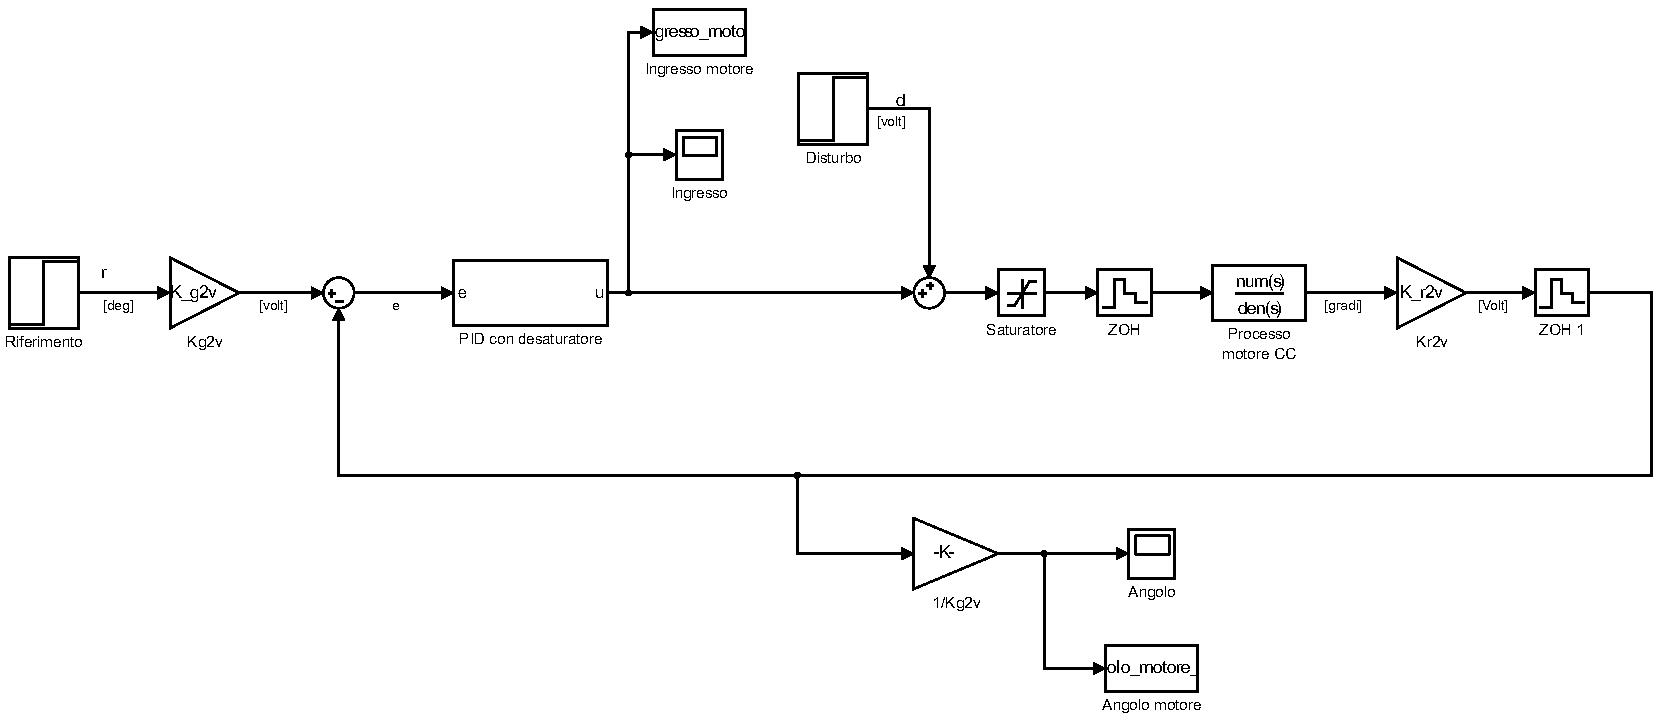
\includegraphics[scale=0.6]{./Figure/SIMULINK/modello_PID.pdf}
		\end{figure}
		
		\paragraph{PID con desaturatore}
		
			\begin{center}
				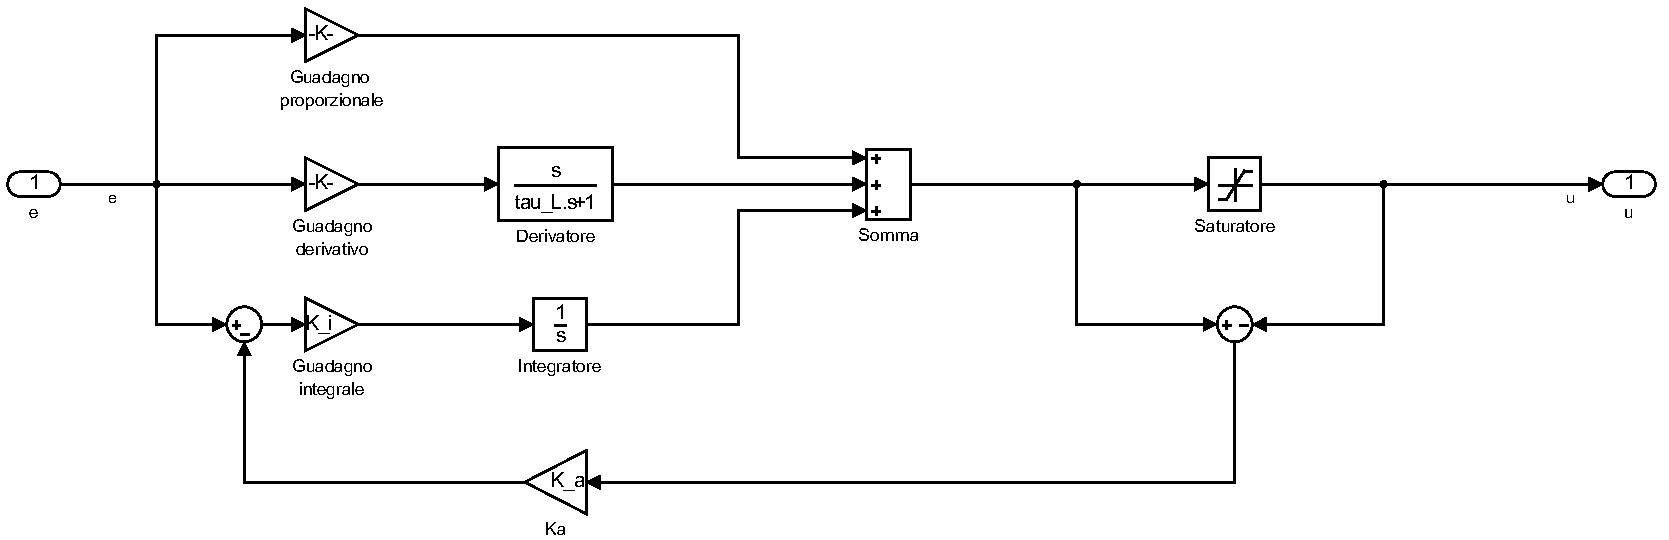
\includegraphics[scale=0.45]{./Figure/SIMULINK/PID_desaturatore.pdf}
			\end{center}
			
	\subsection{modello\_feedforward.slx}
	\label{subapp:modelloFF}
	
		\begin{figure}[H]
			\centering
			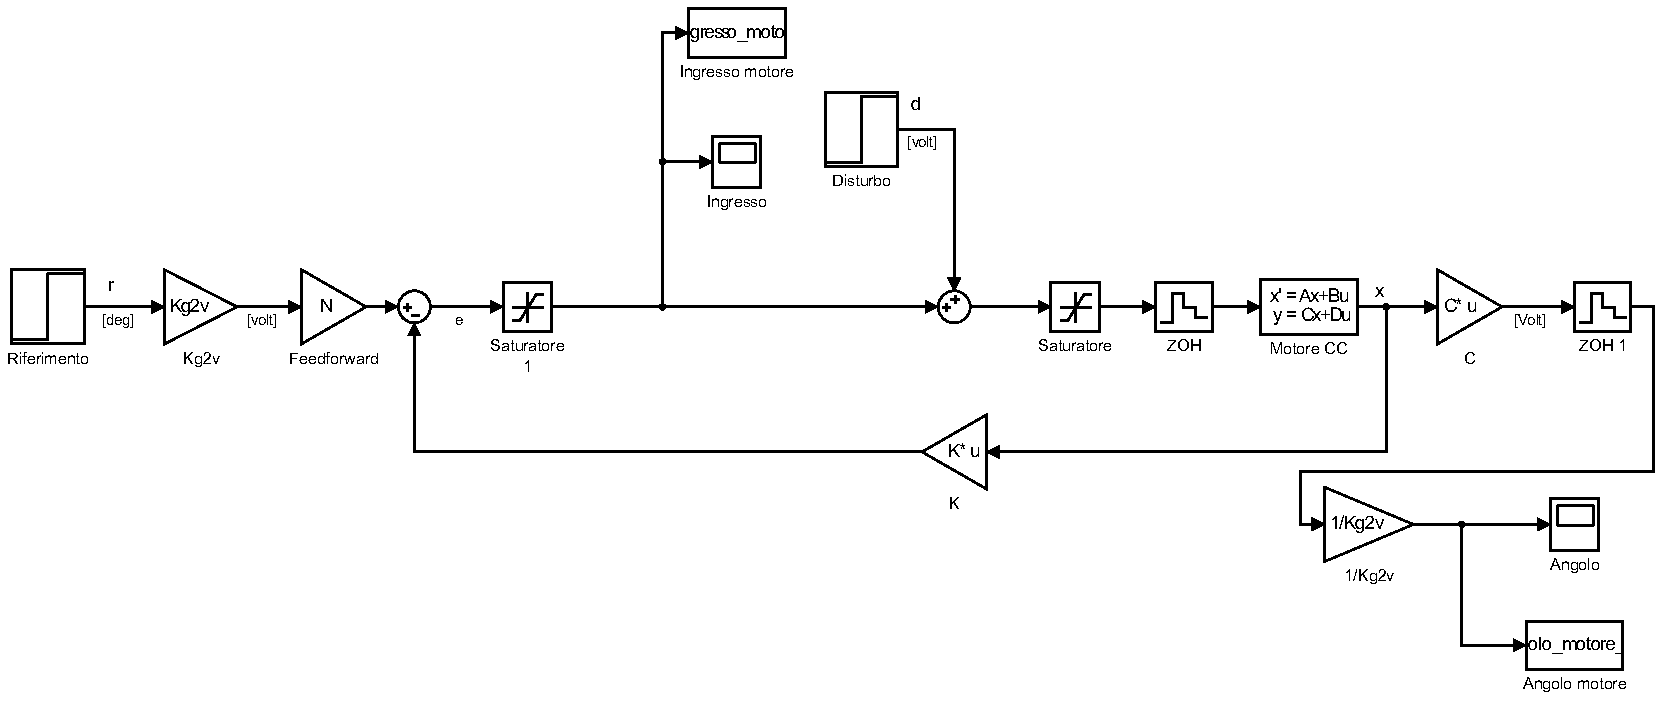
\includegraphics[scale=0.6]{./Figure/SIMULINK/modello_feedforward.pdf}
		\end{figure}			
		
	\subsection{modello\_integrale.slx}
	\label{subapp:modelloIntegrale}
	
		\begin{figure}[H]
			\centering
			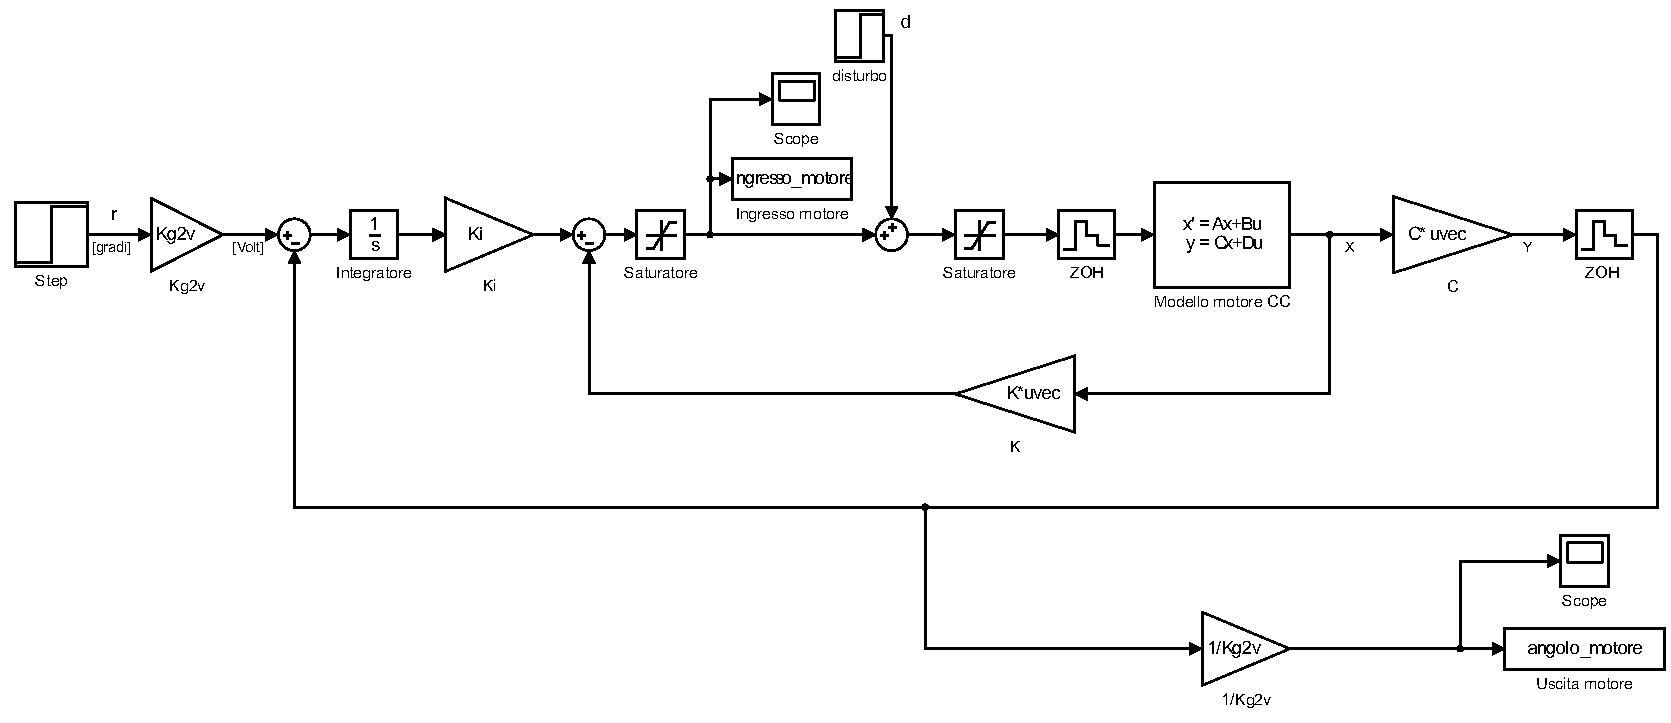
\includegraphics[scale=0.6]{./Figure/SIMULINK/modello_integrale.pdf}
		\end{figure}		
			
		
		
		

		
					

\end{document}

	
